\documentclass[12pt]{article}
\usepackage[utf8]{inputenc}
\usepackage[T1]{fontenc}
\usepackage[brazilian]{babel}
\usepackage{geometry}
\usepackage{graphicx}
\usepackage{amsmath}
\usepackage{amsfonts}
\usepackage{amssymb}
\usepackage{hyperref}
\usepackage{xcolor}
\usepackage{colortbl}
\usepackage{longtable}
\usepackage{booktabs}
\usepackage{array}
\usepackage{listings}
\usepackage{caption}
\usepackage{enumitem}
\usepackage{multirow}
\usepackage{pifont}
\usepackage{float}

\geometry{a4paper, margin=1.5cm}
\hypersetup{colorlinks=true, linkcolor=blue, urlcolor=blue}

% Cores
\definecolor{verde}{RGB}{0,150,0}
\definecolor{azul}{RGB}{0,0,200}
\definecolor{cinza}{RGB}{100,100,100}
\definecolor{vermelho}{RGB}{200,0,0}
\definecolor{amarelo}{RGB}{200,150,0}

% Comandos de status
\newcommand{\ok}{\textcolor{verde}{[\textbf{X}]}}
\newcommand{\pendente}{\textcolor{vermelho}{[\textbf{ }]}}
\newcommand{\andamento}{\textcolor{amarelo}{[\textbf{-}]}}

% Comando para quebra de linha na tabela
\newcommand{\quebra}{\newline}

\title{
    \Huge\textbf{Jogo Bruxa} \\
    \Large Documento de Design
}
\author{}
\date{}

\begin{document}

\maketitle

\begin{center}
\large \textit{Jogo narrativo de alquimia e decisoes entre o mundo dos vivos e dos mortos.}
\end{center}

\tableofcontents

\newpage



\section{Informacoes do Projeto}

\begin{tabular}{|l|l|}
\hline
\textbf{Propriedade} & \textbf{Valor} \\
\hline
Engine & Godot 4 \\
Plataforma & Android \\
Resolucao & 640 x 960 px \\
Genero & Point \& Click \\
Estilo & Side-scroller \\
\hline
\end{tabular}


\section{Layout da Tela}

\begin{verbatim}
Tela (640x960)

+--------------------------+
|                          |
|    Cena (640x640)        |
|                          |
|                          |
|                          |
|                          |
|                          |
|                          |
|         (60%)            |
|                          |
+--------------------------+
|        HUD (40%)         |
|                          |
|               |          |
| Texto  60%    |Opcoes 40%|
|               |          |
+--------------------------+
\end{verbatim}



\newpage
\section{Estrutura de Jogo (em progresso)}

\begin{verbatim}
MAIN
|
+-- GameManager [X] (game_manager.gd - funcionando)
|   +-- DatabaseManager [X] (database_manager.gd - lendo JSON)
|   +-- AudioManager [ ] (vazio)
|   +-- Interpeter [ ] (vazio)
|   +-- GameTemp [X] (estado: vars, pers, inventario)
|
+-- CanvasLayer
|   +-- HUD [X] (visivel)
|   |   +-- Inventario [X] (estrutura pronta) 
|   |   |   |   Obs: inventario visivel o tempo todo,
|   |   |   |   com scroll de uma lista horizontal
|   |   |   +-- Panel [X]
|   |   |   +-- GridContainer [-] (Slots 1 e 2) 
|   |   |   |   Obs: trocara para lista horizontal
|   |   |   +-- InfoItem [X] (Label)
|   |   |   +-- TextureRect [X] (frame.png)
|   |   +-- ColorRect2 [X] (fundo cinza)
|   |   +-- Label [X] (Bruxa stats)
|   |
|   +-- PauseMenu [X] (visivel)
|   |   +-- Background [X]
|   |   +-- VBoxContainer [X]
|   |   |   +-- Continuar [X] (conectado ao GameManager)
|   |   |   +-- Opcoes [ ] (sem funcao)
|   |   |   +-- Sair [X] (conectado ao GameManager)
|   |   +-- Label [X] (atualizado com dados do DB)
|   |
|   +-- Notificacao [X] (estrutura pronta)
|   |   +-- Container -> NotificacaoItem [X] (Panel)
|   |
|   +-- CenaPreparo [ ] (invisivel)
|   |   +-- Background [ ]
|   |   +-- CenterContainer [ ]
|   |   |   +-- VBoxContainer [ ]
|   |   |       +-- Animation [ ]
|   |   |       +-- Graph [ ]
|   |   |       +-- HBoxContainer [ ]
|   |   |           +-- LeftButton [ ]
|   |   |           +-- ListaHorizontal [ ]
|   |   |           +-- RightButton [ ]
|   |   +-- Label [ ]
|   |
|   +-- MenuPrincipal [ ] (invisivel)
|       +-- TextureRect [ ]
|       +-- VBoxContainer [ ]
|       |   +-- Iniciar [ ]
|       |   +-- Carregar [ ]
|       |   +-- Opcoes [ ]
|       |   +-- Sair [ ]
|       +-- Label [ ]
|       +-- Label2 [ ]
|
+-- Mundo [X] (visivel)
    +-- Player [X] (estrutura pronta)
    |   +-- Camera2D [X]
    |   +-- Sprite2D [X] (player_parado.png)
    |   +-- CollisionShape2D [X]
    |   +-- AnimationTree [X]
    |   +-- AnimationPlayer [X]
    +-- MapaFlorestaA [X] (instancia carregada)
\end{verbatim}


\subsection{Conexoes}

\begin{verbatim}
Continuar (pressed) -> GameManager._on_continuar_pressed
Sair (pressed)      -> GameManager._on_sair_pressed
DatabaseManager.loaded -> GameTemp._on_database_loaded
\end{verbatim}


\subsection{Status dos Modulos}

\begin{table}[h]
\centering
\small
\begin{tabular}{|l|c|p{5cm}|p{2.5cm}|}
\hline
\textbf{Modulo} & \textbf{Status} & \textbf{Observacao} & \textbf{Prioridade} \\
\hline
GameManager & [X] & Gerenciando tudo & - \\
DatabaseManager & [X] & Lendo JSON com sucesso & - \\
GameTemp & [X] & Estado do jogo funcionando & - \\
HUD/Inventario & [X] & Estrutura visual pronta & - \\
PauseMenu & [X] & Continuar e Sair funcionando & - \\
Notificacao & [X] & Estrutura pronta p/ mensagens & - \\
Player & [X] & Estrutura pronta p/ movimento & - \\
\hline
AudioManager & [ ] & Vazio & Alta \\
Interpeter & [ ] & Vazio & Alta \\
MenuPrincipal & [ ] & Invisivel, sem funcao & Alta \\
CenaPreparo & [ ] & Invisivel, sem funcao & Media \\
Opcoes & [ ] & Sem funcao & Baixa \\
Editor de GameTemp & [ ] & - & Media \\
\hline
\end{tabular}
\caption{Status de Desenvolvimento}
\end{table}

\newpage

\section{Mapa}

\subsection{Links MIRO}

\begin{itemize}
    \item Capitulo 1: \url{https://miro.com/app/board/uXjVHHRQsyM=/}
    \item Capitulo 2: (em breve)
    \item Capitulo 3: (em breve)
\end{itemize}

\subsection{Relações do Mapa}

\scriptsize
\begin{longtable}{|c|p{2.2cm}|p{1.5cm}|p{2cm}|p{2.5cm}|p{2.5cm}|p{2.8cm}|}
\hline
\textbf{ID} & \textbf{Cena} & \textbf{Dim.} & \textbf{Conecta} & \textbf{Funcao} & \textbf{Elementos} & \textbf{Objetivo} \\
\hline
1 & Floresta & 8000 & 1.1, 2, 7 & Exploracao princ. & Arvores, ervas, ingredientes & Coletar recursos e avancar \\
1.1 & BruxaOut & 1280 & 1, 1.1.1 & Area externa base & Casa, arvore, jardim & Acessar a casa ou retornar \\
1.1.1 & BruxaIn & 1280 & 1.1 & Base inicial & Caldeirao, mesa, alquimia & Criar pocoes \\
\hline
2 & Bosque & 2000 & 1, 3 & Area de transicao & Vegetacao aberta & Chegar a cidade \\
\hline
3 & CidadeA & 5000 & 2, 3.1, 3.2, 3.3, 4 & Hub social & NPCs, casas, lojas & Conversar e receber missoes \\
3.1 & CasaNPC1 & 1280 & 3 & Interior NPC & Comerciante/morador & Obter itens/informacoes \\
3.2 & CasaNPC2 & 1280 & 3 & Interior NPC & Morador/alquimista & Descbloquear recompensas \\
3.3 & CasaNPC3 & 1280 & 3 & Interior NPC & Plebeu doente da missão & Completar missao \\
\hline
4 & Estrada & 2000 & 3, 5 & Estrada principal & Caminho aberto & Prosseguir a ponte \\
\hline
5 & Ponte & 2000 & 4, 6 & Evento interm. & Ponte, rio, item 1/2 para poção ansiolítica. Guarda& Superar desafio \\
\hline
6 & CasteloOut & 3000 & 5, 6.1, 7 & Exterior castelo & Muralhas, portao & Entrar no castelo \\
6.1 & CasteloIn & 2500 & 6 & Climax & Saloes, guardas, chefe & Concluir missao principal \\
\hline
7 & EstradaSec. & 3000 & 1, 6 & Atalho & Caminho alternativo, item 2/2 para poção ansiolítica. Guarda & Acesso rapido ao castelo \\
\hline
\caption{Mapa de Cenas e Conexoes}
\end{longtable}
\normalsize

\begin{figure}[htbp]
    \centering
    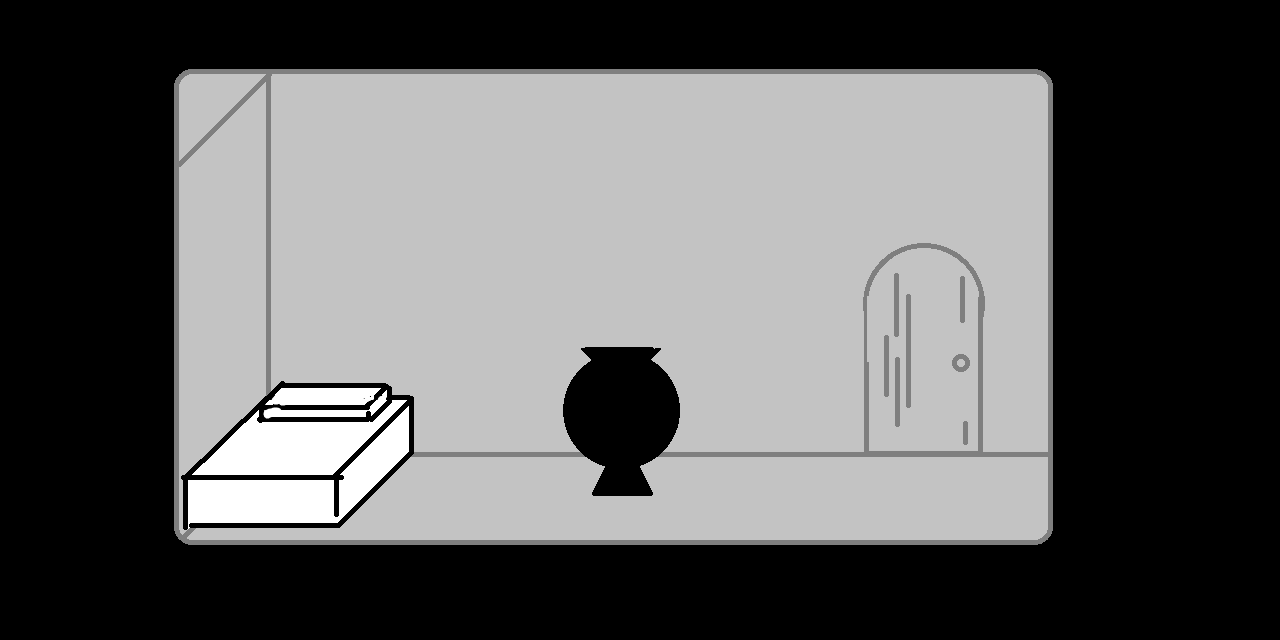
\includegraphics[width=1.0\textwidth]{img/mapa_bruxa_in_bg.png}
    \caption{Mapa Bruxa In}
    \label{fig:mapa_bruxa_in}
\end{figure}

\begin{figure}[htbp]
    \centering
    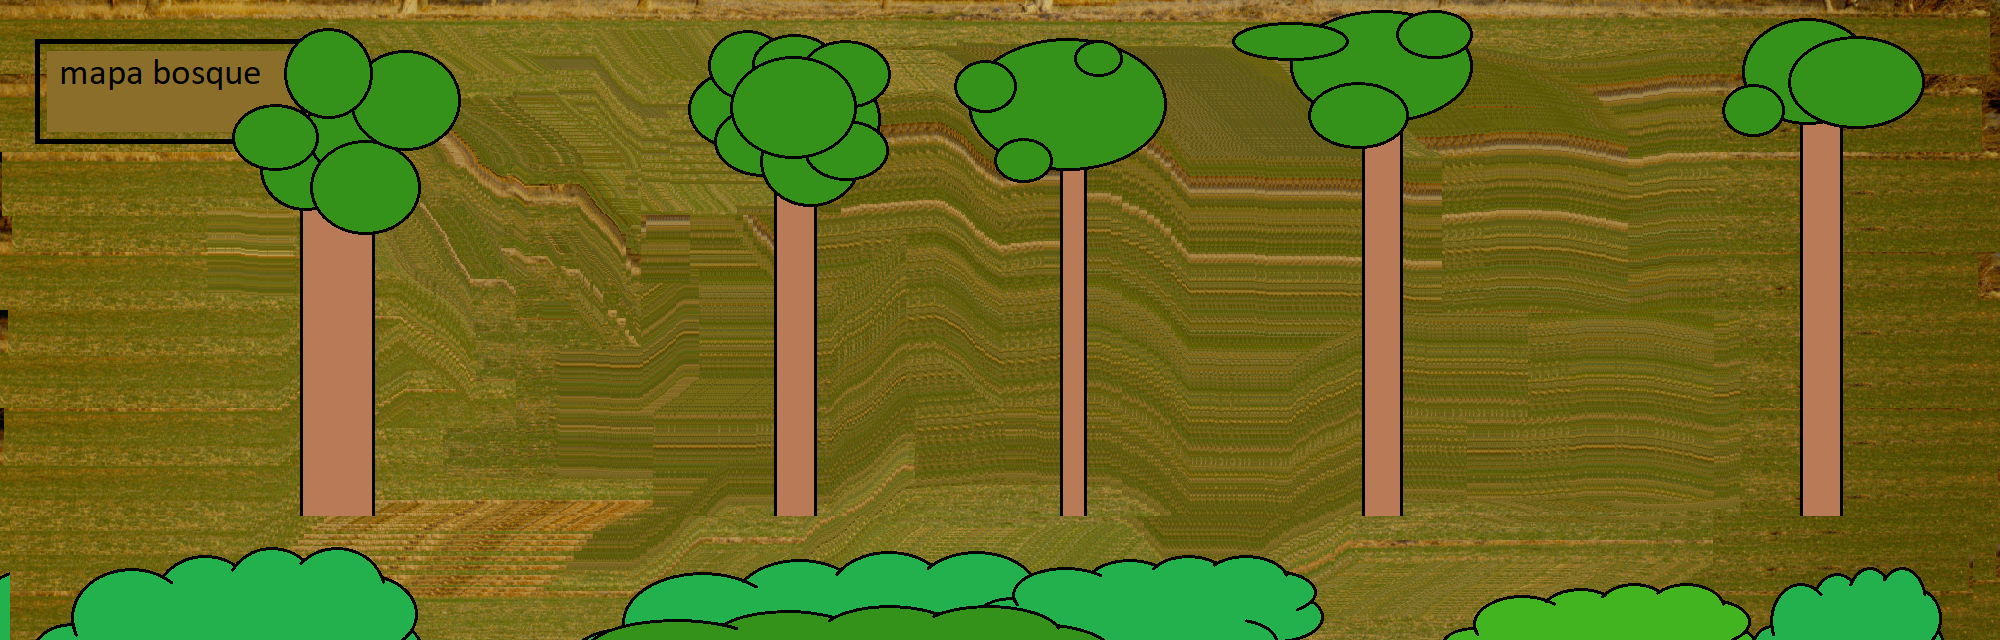
\includegraphics[width=1.0\textwidth]{img/mapa_bosque.png}
    \caption{Mapa do Bosque}
    \label{fig:mapa_bosque}
\end{figure}

\begin{figure}[htbp]
    \centering
    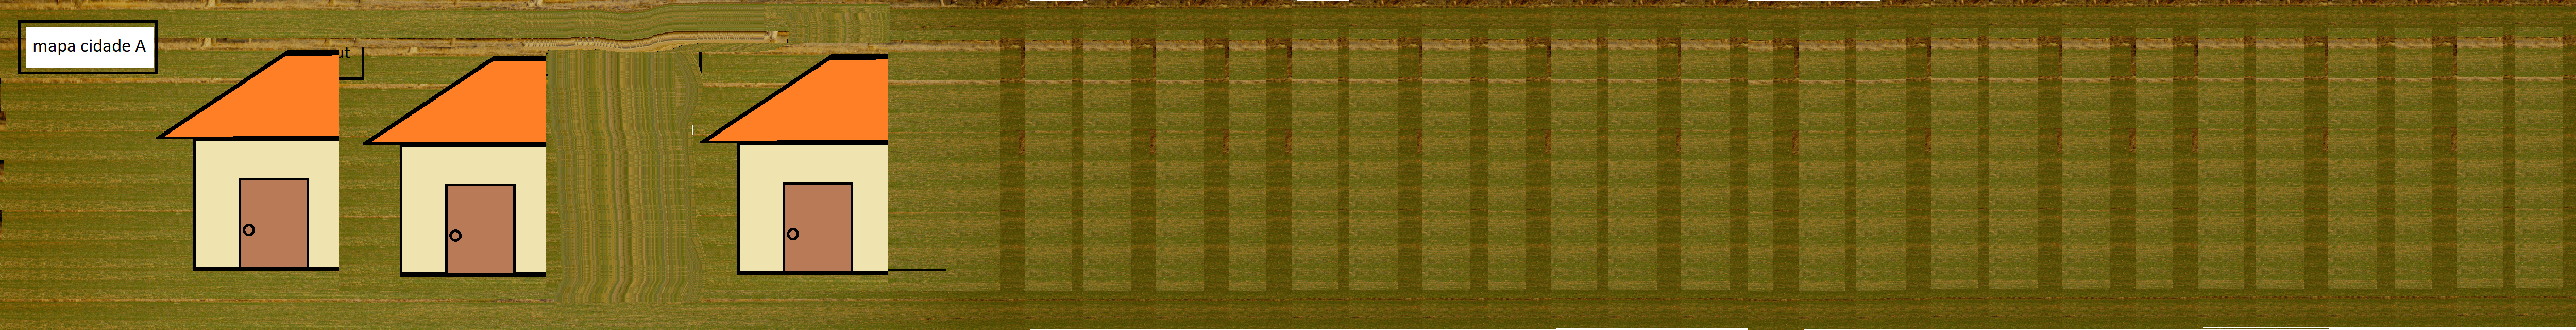
\includegraphics[width=1.0\textwidth]{img/mapa_cidade_A.png}
    \caption{Mapa Cidade A}
    \label{fig:mapa_cidadeA}
\end{figure}

\begin{figure}[htbp]
    \centering
    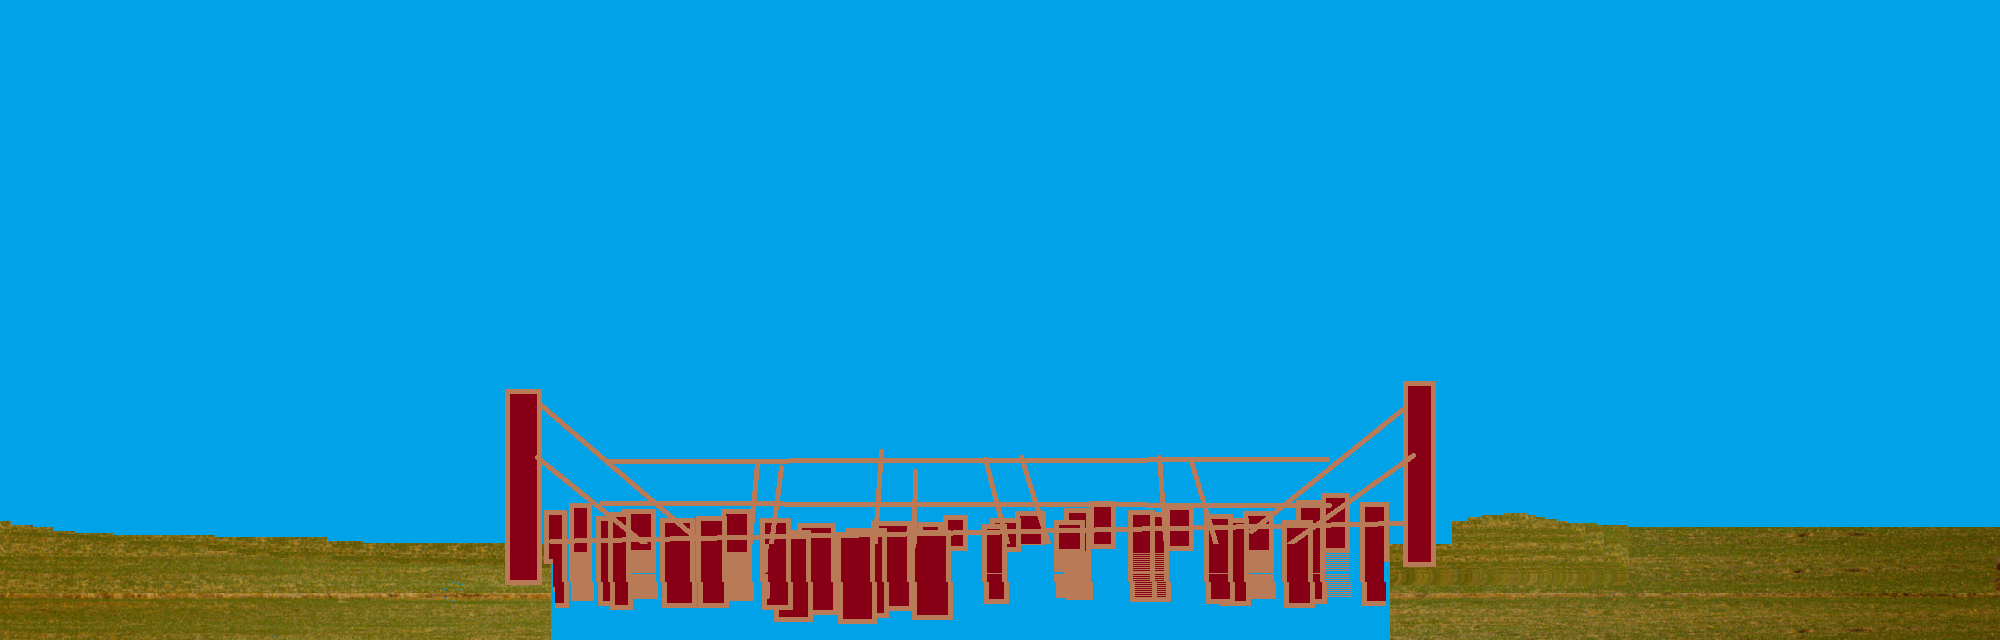
\includegraphics[width=1.0\textwidth]{img/mapa_ponte.png}
    \caption{Mapa da Ponte}
    \label{fig:mapa_ponte}
\end{figure}


\begin{figure}[htbp]
    \centering
    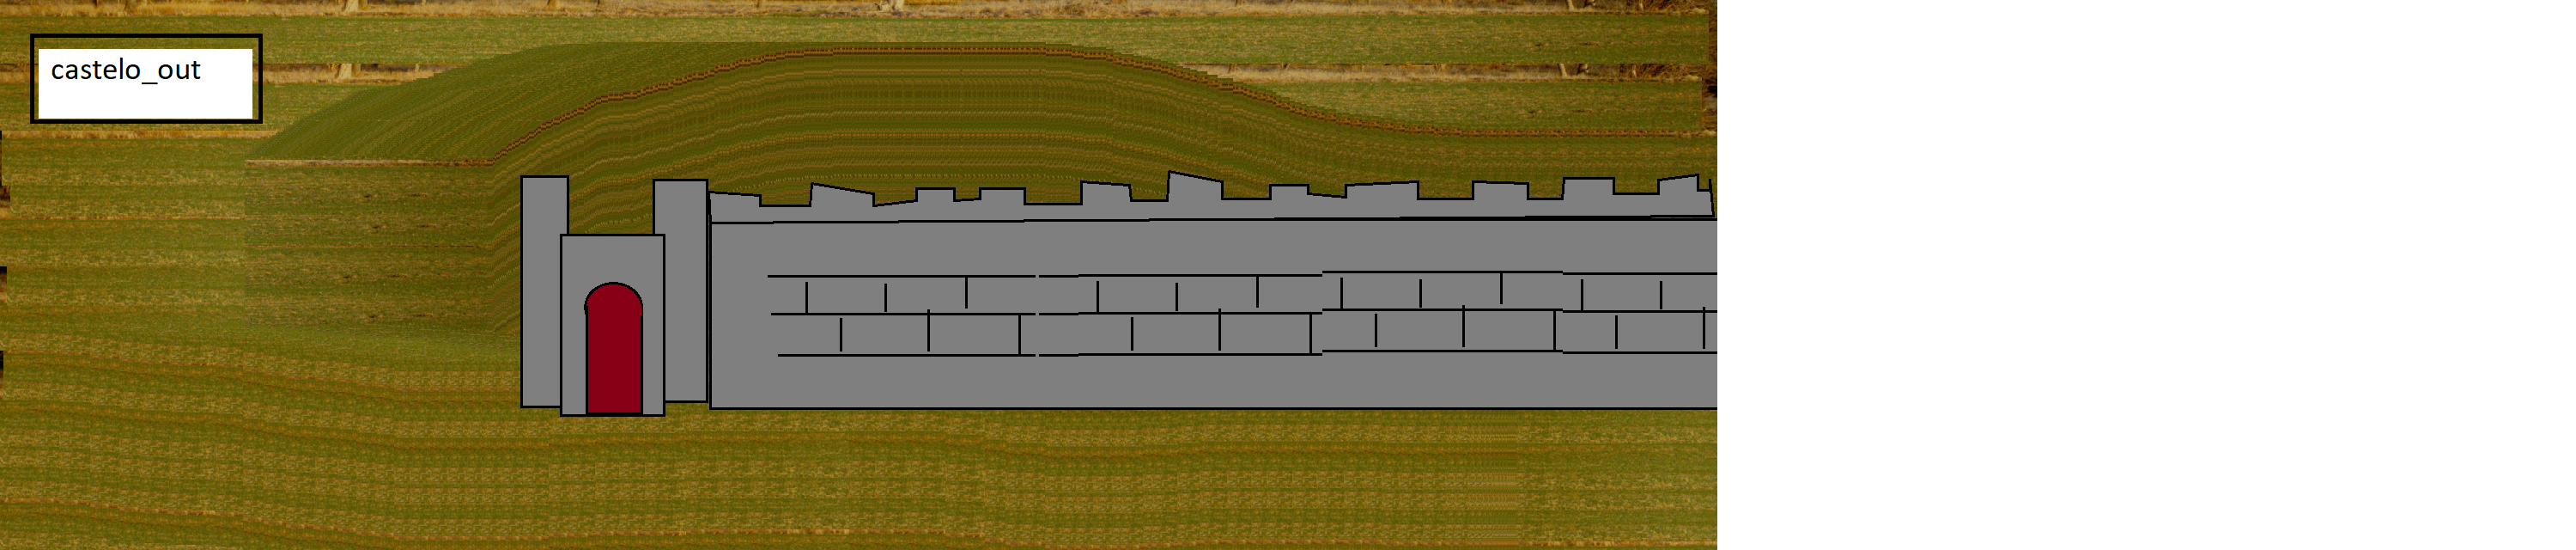
\includegraphics[width=1.5\textwidth]{img/mapa_castelo_out.png}
    \caption{Mapa do Castelo Out}
    \label{fig:mapa_cast_out}
\end{figure}





\newpage

\section{Historia}

\subsection{Contexto / Mundo}

\textbf{Cenario:} Europa Medieval

\vspace{0.3cm}

\noindent Entre o mundo dos vivos e o mundo dos mortos existe um fino veu que os separa. Para a maioria das pessoas esse veu e imperceptivel, mas aqueles que tem contato com a magia podem ver atraves.

\vspace{0.2cm}

\noindent A cada dia que passa o mundo dos mortos esta mais cheio e alguns espiritos, por vontade ou acaso, acabam chegando tao perto do veu que interferem no mundo dos vivos.

\vspace{0.2cm}

\noindent A Bruxa [\ldots\ldots\ldots\ldots], se mudou para perto da cidade a pouco tempo, ela veio para descansar. Porem, os mortos e vivos tem problemas diversos e ficam te chamando toda hora para fazer pocoes para eles.

\vspace{0.2cm}

\noindent Para as pocoes sao necessarios ingredientes de lugares diversos, entao a bruxa resolveu pendurar na sua porta, um pedaco do veu entre mundos, assim nao precisara perder tempo ou importar ingredientes caros.

\vspace{0.2cm}

\noindent Foram 4 dias para a criacao da casa. Um dia para cortar as madeiras. Outro para montar a casa. Um dia para pegar um pedaco do veu. E o ultimo dia, para preparar os moveis e encantamentos. Assim a casa estava pronta e a bruxa pode descansar.

\subsection{Introducao}

\textbf{Cenario:} Casa da bruxa (na floresta), manha com nevoa.

\vspace{0.3cm}

\begin{quote}
\itshape
A neblina ainda danca entre os pinheiros quando os primeiros sinos de argila pendurados na porta soam. Por dentro da casa, frascos coloridos repousam em prateleiras tortas, raizes secando pendem do teto, e um caldeirao fumegante com uma mistura esverdeada. O cheiro e de hortela, enxofre e terra umida.

\vspace{0.3cm}

\noindent Voce, a bruxa, esta proxima a mesa, enrolando rabos de salamandra quando a porta se abre com um rangido lento. Um jovem campones entra, com chapeu nas maos e os olhos baixos.

\vspace{0.3cm}

\noindent "Dona… minha irma vai se casar amanha, mas ela perdeu a voz. Pode nos ajudar?"
\end{quote}

\vspace{0.3cm}

\noindent Voce se levanta, pega um livro pesado com fecho de ossos e o abre sobre a mesa. A luz das velas tremula. Um menu aparece com ingredientes possiveis: mel de fada, lingua de tritao, eco de caverna, orvalho de flor da manha, etc.

\newpage

\subsection{Capitulo 1}

\begin{itemize}[leftmargin=*]
    \item \textbf{Cenário:} Floresta /  Bosque / Cidade A / Estradas / Ponte / Castelo
    \item \textbf{Missão:} Pegar ingredientes, criar poção, curar doença de ansiedade no plebeu, pegar a carta validando, depois curar a mesma doença na princesa.
    \item \textbf{Roteiro:} Bruxa em casa, vem pessoa avisar doença num plebeu, bruxa vai ver ela na cidade, bruxa pega itens, bruxa cozinha, bruxa volta no plebeu doente, aplica poção, reação, carta para o rei, bruxa vai na guarda, bruxa vai no rei, aplica poção na princesa.
    \item \textbf{Menor caminho:} $1.1.1\rightarrow1.1\rightarrow1\rightarrow2\rightarrow3\rightarrow3.3\rightarrow3\rightarrow4\rightarrow5\rightarrow4\rightarrow3\rightarrow2\rightarrow1\rightarrow7\rightarrow1\rightarrow1.1\rightarrow1.1.1\rightarrow1.1\rightarrow1\rightarrow2\rightarrow3\rightarrow3.3\rightarrow3\rightarrow4\rightarrow5\rightarrow6\rightarrow6.1$
\end{itemize}

\subsection{Entre capítulos (mais curto)}

\begin{itemize}[leftmargin=*]
    \item \textbf{Cenario:} Casa da Bruxa / Véu
    \item \textbf{Missao:} Aprender a usar a porta
    \item \textbf{Roteiro:} Um pedido de poção de um ingrediente que só tem no mar(ou outro ambiente), a bruxa abre a porta para o véu
\end{itemize}

\subsection{Capitulo 2}

(introvertido vs extrovertido)

\begin{itemize}[leftmargin=*]
    \item \textbf{Cenario:} Cidade B
    \item \textbf{Missao:} (em desenvolvimento)
    \item \textbf{Roteiro:} (em desenvolvimento)
\end{itemize}

\subsection{Capitulo 3}

(epidemia de ansiedade)

\begin{itemize}[leftmargin=*]
    \item \textbf{Cenario:} Mundo dos Mortos
    \item \textbf{Missao:} Enganar o diabo, eventos ambiguos
    \item \textbf{Roteiro:} (em desenvolvimento)
\end{itemize}

\newpage

\section{Fluxo de Missoes}

\begin{verbatim}
Idle
 v
Visitante chega
 v
Historia (poucas msgs)
 v
Investigar/Pegar ingredientes (dialogo, NPC, livro, ...)
 v
Criacao de pocao
 v
Aplicação (curar/falhar)
 v
Conclusao
 v
Idle
\end{verbatim}


\newpage
\section{Mecanicas}

\paragraph{Oficiais}

\begin{itemize}
    \item Sistema de preparar pocoes
    \item Diálogo e Escolhas com consequencias
    \item Várias portas dão numa mesma porta
    \item Personalidades
\end{itemize}

\paragraph{Brainstorm (mecanicas possiveis)}

\begin{verbatim}
-----------------------------------------------------
Legenda (ordem de prioridade):
(-1) = fazer urgente
(0) = fazer logo
(1) = fazer depois do cap 1
(2) = fazer depois do cap 2
(...)
-----------------------------------------------------
(-1) 
- implementar sistemas basicos (dialogo, escolhas, 
  preparo pocao, interacao, save) 
- fazer testes ostensivos

(0) 
- terminar cap 1 

(1)
- Clima / tempo corrido
- Economia (compra/venda ou valor dinamico, desvalorização)
- Fama / inveja
- Equipamentos de alquimia
- HP
- Personalidade de todos seres

(2)
- NPCs auxiliares
- FadeOut/In circular com raio crescendo/descrescendo
\end{verbatim}

\subsection{Poções e Personalidades}

\begin{figure}[htbp]
    \centering
    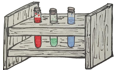
\includegraphics[width=0.25\textwidth]{img/mapa_bruxa_in_pocoes.png}
    \caption{Poções}
    \label{fig:mapa_bruxa_in_pocoes}
\end{figure}

O estado da personalidade de uma pessoa é representado por um vetor em \(\mathbb{R}^5\):

\[
x \in \mathbb{R}^5
\]

As poções são itens que modificam uma personalidade, são representados por uma matriz $A$:

\[A : \text{matriz 5x5}\]


A nova personalidade $p$, após o uso da poção, é calculada por:

\[
p(x) = Ax + b
\]

Onde:
\begin{itemize}
    \item \(x \in \mathbb{R}^5\) é a personalidade que será mudada
    \item \(A \in \text{Mat}_5(\mathbb{R})\) é a matriz de transformacao da poção
    \item \(b \in \mathbb{R}^{5}\) são um termo de erro adicionado
\end{itemize}



\subsubsection{Preparo de Poções}


O preparo de poções se dá ao combinar ingredientes e controlar a temperatura e tempo de cozimento.


[IMG TELA DE PREPARO]***
\paragraph{Layout}
- Animação
- 

\paragraph{Temperatura}
Início: 20°C

\paragraph{Tempo}
Quando a bruxa coloca o primeiro ingrediente, a receita é iniciada.

\paragraph{Ingredientes}

Os ingredientes são os componentes que combinados geram uma poção. 
Cada ingrediente tem sua matriz $A$ e sua temperatura de cozimento $\mu $.

\begin{itemize}
    \item \(A\) matrix 5x5
    \item \(\mu\) temperatura de cozimento média
    \item \(\sigma\) desvio padrão de cozimento
\end{itemize}

\paragraph{Preparo}

O caldeirão começa com a matriz $A=I_{5x5}$ representando a água.
O fogo sempre tende a ficar na temperatura ambiente.
A bruxa pode aumentar o fogo abanando.
Ao colocar o primeiro ingrediente a receita começa.
Cada ingrediente tem sua potencia ideal de cozimento.
Se fugir muito da potencia ideal, não se aproveita ao máximo seus atributos. 
A ordem dos ingredientes importa e eles são adicionados um a um.
A receita só para quando a bruxa decidir retirar do caldeirão.


Ao final é calculada a matriz $A$ da poção gerada:

\[A = \prod{\alpha_i A_i} = (\prod{\alpha_i}) \cdot \prod{A_i} \]
\[i \leq n \]

sua qualidade $\alpha$ é calculada a partir da média dos $\alpha_i$.



\begin{table}[H]
\centering
\caption{Principais classes de matrizes dos ingredientes}
\renewcommand{\arraystretch}{1.3}
\begin{tabular}{|l|l|c|l|}
\hline
\textbf{Categoria} & \textbf{Classe} & \textbf{Notação} & \textbf{Caracterização} \\
\hline
\multirow{6}{*}{Estrutural}
& Simétrica           & $A=A^T$               & Igual à transposta. \\ \cline{2-4}
& Diagonal            & $a_{ij}=0,\ i\neq j$  & Apenas a diagonal principal pode ser não nula. \\ \cline{2-4}
& Definida positiva   & $x^TAx>0$             & $\forall\,x\neq0$. \\ \cline{2-4}
& Antissimétrica      & $A=-A^T$              & Diagonal principal nula. \\ \cline{2-4}
& Ortogonal           & $A^TA=I$              & $A^{-1}=A^T$. \\ \cline{2-4}
& Permutação          & $P^TP=I$              & Ortogonal com entradas $0$ ou $1$. \\
\hline
\multirow{5}{*}{Polinomial}
& Idempotente         & $A^2=A$               & Projeção. \\ \cline{2-4}
& Involutória         & $A^2=I$               & É sua própria inversa. \\ \cline{2-4}
& Nilpotente          & $A^k=0$               & Para algum $k\ge1$. \\ \cline{2-4}
& Periódica           & $A^k=I$               & Para algum $k\ge1$. \\ \cline{2-4}
& Potência-estável    & $A^m=A$             & Para alguns $,\ge1$. \\
\hline
\end{tabular}
\end{table}
\paragraph{Simétrica}
Ingredientes simétricos produzem efeitos previsíveis e estáveis(?)***. São os mais fáceis de combinar com outros ingredientes, pois sua transformação não introduz distorções inesperadas.

\paragraph{Definida positiva}
Ingredientes definidos positivos sempre fortalecem algum aspecto da personalidade, nunca a anulando ou invertendo. São considerados ingredientes seguros e de alta qualidade.

\paragraph{Antissimétrica}
Ingredientes antissimétricos redistribuem traços de personalidade entre si sem aumentar ou diminuir significativamente a intensidade total. São úteis para equilibrar extremos.

\paragraph{Ortogonal}
Ingredientes ortogonais preservam a intensidade da personalidade, modificando apenas sua direção. Em outras palavras, transformam a personalidade sem enfraquecê-la nem fortalecê-la.

\paragraph{Permutação}
Ingredientes de permutação apenas trocam características de lugar. Por exemplo, podem transformar desprezo em curiosidade ou introversão em abertura criativa, preservando os valores originais.

\paragraph{Idempotente}
Após usar uma vez, adicionar novamente o mesmo ingrediente não produz efeito adicional. Assim, ingredientes idempotentes possuem um efeito de saturação natural só com 2 usos.

\paragraph{Involutória}
Ao utilizar o mesmo ingrediente duas vezes consecutivas, a personalidade retorna exatamente ao estado anterior. Esses ingredientes são úteis para desfazer transformações.

\paragraph{Nilpotente}
Os ingredientes de matriz nilpotente são perigosos. Se o mesmo ingrediente for utilizado repetidamente (\(k\) vezes), a poção resultará em uma matriz nula. Como uma matriz nula anula completamente a personalidade, esses ingredientes devem ser manipulados com extremo cuidado.

\paragraph{Periódica}
Ingredientes periódicos apresentam um ciclo de funcionamento. Após um número específico de aplicações, seus efeitos retornam ao estado inicial. Assim, utilizar a quantidade correta pode potencializar a poção, enquanto uma aplicação a mais pode anular completamente o efeito obtido.

\paragraph{Potência-estável}
Após certo número de aplicações, o ingrediente deixa de produzir novos comportamentos. A partir desse ponto, aplicações adicionais apenas repetem estados já observados.

\paragraph{Diagonal}
São as poções de modificação específica. Cada característica da personalidade é alterada independentemente das demais, sem criar interações entre elas. São consideradas poções muito bem refinadas e previsíveis.



\subsection{Interpreter}

O intérprete lida com a fila de comandos dos eventos.

Comandos implementados:

\begin{verbatim}
    [X]  mudar_variavel(id, valor)
    [ ]  mostrar_texto()
    [ ]  mostrar_opcoes()
    [ ]  wait(tempo)
    [ ]  teleport(map_id, x, y, direcao)
    [ ]  tocar_som(nome, vol)
    [ ]  tocar_musica(nome, vol)
    [ ]  mudar_item(id, qtd)
    [ ]  mudar_personalidade(id, novo_p)
    [ ]  camera_mover(pos, tempo)
    [ ]  camera_tremer(intensidade, freq, tempo)
    [ ]  chamar_evento(id, forcar_pagina) 
    [ ]  mover_player(posicao, tempo)
    [ ]  mover_evento(id, posicao, tempo)
    [ ]  mudar_cor_tela(cor, tempo)
    [ ]  mostrar_animacao() ??
    [ ]  if / else (condicao)
    [ ]  while(condicao)
\end{verbatim}

\newpage
\end{document}